%! suppress = MissingLabel
\documentclass[12pt,letterpaper,oneside,reqno]{amsart}
\usepackage{amsfonts}
\usepackage{amsmath}
\usepackage{amssymb}
\usepackage{amsthm}
\usepackage{float}
\usepackage{mathrsfs}
\usepackage{colonequals}
\usepackage[font=small,labelfont=bf]{caption}
\usepackage[left=1in,right=1in,bottom=1in,top=1in]{geometry}
\usepackage[pdfpagelabels,hyperindex,colorlinks=true,linkcolor=blue,urlcolor=magenta,citecolor=green]{hyperref}
\usepackage{graphicx}
\linespread{1.7}
\emergencystretch=1em
\usepackage{array}
\usepackage{etoolbox}
\apptocmd{\sloppy}{\hbadness 10000\relax}{}{}
\raggedbottom

\newcommand \anglePower [2]{\langle #1 \rangle \sp{#2}}
\newcommand \bernoulli [2][B] {{#1}\sb{#2}}
\newcommand \curvePower [2]{\{#1\}\sp{#2}}
\newcommand \coeffA [3][A] {{\mathbf{#1}} \sb{#2,#3}}
\newcommand \polynomialP [4][P]{{#1}(#2,#3,#4)}
\newcommand \polynomialQ [4][Q]{{#1}(#2,#3,#4)}

% ~~~ Rascal numbers ~~~
%\newcommand \rascalNumber [3] {\binom{#1}{#2}_{#3}}
%\newcommand \north[0] {\mathbf{North}}
%\newcommand \south[0] {\mathbf{South}}
%\newcommand \west[0] {\mathbf{West}}
%\newcommand \east[0] {\mathbf{East}}

% ~~~~ 1-q pascal notation~~~~
%\newcommand{\genstirlingI}[3]{%
%    \genfrac{[}{]}{0pt}{#1}{#2}{#3}%
%}
%\newcommand{\genstirlingII}[3]{%
%    \genfrac{\{}{\}}{0pt}{#1}{#2}{#3}%
%}
%\newcommand{\oneQBinomial}[3]{\genstirlingI{}{#1}{#2}^{#3}}

% free foot note
%\let\svthefootnote\thefootnote
%\newcommand\freefootnote[1]{%
%    \let\thefootnote\relax%
%    \footnotetext{#1}%
%    \let\thefootnote\svthefootnote%
%}


\newtheorem{theorem}{Theorem}[section]
\newtheorem{corollary}[theorem]{Corollary}
\newtheorem{lemma}[theorem]{Lemma}
\newtheorem{example}[theorem]{Example}
\newtheorem{conjecture}[theorem]{Conjecture}
\newtheorem{definition}[theorem]{Definition}

%\numberwithin{equation}{section}

\title[Plots of Closed Forms]
{Plots of Closed Forms}
\author[Petro Kolosov]{Petro Kolosov}
%\address{Software Developer, DevOps Engineer}
%\email{kolosovp94@gmail.com}
%\urladdr{https://kolosovpetro.github.io}
%\keywords{
%    Binomial theorem,
%    Binomial coefficients,
%    Faulhaber's formula,
%    Polynomials,
%    Pascal's triangle
%    Finite differences,
%    Interpolation,
%    Polynomial identities
%}
%\subjclass[2010]{26E70, 05A30}
%\date{\today}
\hypersetup{
    pdftitle={Plots of Closed Forms},
    pdfsubject={
        Polynomials,
        Finite differences,
        Interpolation,
        Approximation,
        Polynomial identities,
        Power sums,
        Binomial theorem,
        Power function,
        Binomial coefficients,
        Bernoulli numbers,
        Pascal's triangle,
        Faulhaber's formula,
        Derivatives,
        Differential calculus,
        Partial differential equations,
        OEIS,
        Bernoulli polynomials,
        Combinatorics,
        Discrete convolution,
        Dynamic systems,
        Time scales
    },
    pdfauthor={Petro Kolosov},
    pdfkeywords={
        Polynomials,
        Finite differences,
        Interpolation,
        Approximation,
        Polynomial identities,
        Power sums,
        Binomial theorem,
        Power function,
        Binomial coefficients,
        Bernoulli numbers,
        Pascal's triangle,
        Faulhaber's formula,
        Derivatives,
        Differential calculus,
        Partial differential equations,
        OEIS,
        Bernoulli polynomials,
        Combinatorics,
        Discrete convolution,
        Dynamic systems,
        Time scales
    }
}
\begin{document}
%    \begin{abstract}
%        Your abstract here.
%    \end{abstract}

    \maketitle

    \tableofcontents

%    \freefootnote{Sources: \url{https://github.com/kolosovpetro/github-latex-template}}

    \section{Introduction}\label{sec:introduction}
    \begin{align*}
        \polynomialP{m}{X}{N} &= \sum_{r=0}^{m} \sum_{k=1}^{N} \coeffA{m}{r} k^r (X-k)^r \\
        \polynomialQ{m}{X}{N} &= \sum_{r=0}^{m} \sum_{k=0}^{N-1} \coeffA{m}{r} k^r (X-k)^r
    \end{align*}

    \begin{align*}
        \polynomialP{m}{N}{N} &= N^{2m+1} \\
        \polynomialQ{m}{N}{N} &= N^{2m+1} \\
        \polynomialP{m}{N+1}{N} &= (N+1)^{2m+1} - 1 \quad \quad (verified) \\
        \polynomialQ{m}{N-1}{N} &= (N-1)^{2m+1} + 1 \quad \quad (verified)
    \end{align*}

    \subsection{Polynomials P(1,X,N) N = 1 to 20}
    
\begin{align*}
    \polynomialP{1}{X}{0} &= 0 \\
    \polynomialP{1}{X}{1} &= 6X - 5 \\
    \polynomialP{1}{X}{2} &= 18X - 28 \\
    \polynomialP{1}{X}{3} &= 36X - 81 \\
    \polynomialP{1}{X}{4} &= 60X - 176 \\
    \polynomialP{1}{X}{5} &= 90X - 325 \\
    \polynomialP{1}{X}{6} &= 126X - 540 \\
    \polynomialP{1}{X}{7} &= 168X - 833 \\
    \polynomialP{1}{X}{8} &= 216X - 1216 \\
    \polynomialP{1}{X}{9} &= 270X - 1701 \\
    \polynomialP{1}{X}{10} &= 330X - 2300 \\
    \polynomialP{1}{X}{11} &= 396X - 3025 \\
    \polynomialP{1}{X}{12} &= 468X - 3888 \\
    \polynomialP{1}{X}{13} &= 546X - 4901 \\
    \polynomialP{1}{X}{14} &= 630X - 6076 \\
    \polynomialP{1}{X}{15} &= 720X - 7425 \\
    \polynomialP{1}{X}{16} &= 816X - 8960 \\
    \polynomialP{1}{X}{17} &= 918X - 10693 \\
    \polynomialP{1}{X}{18} &= 1026X - 12636 \\
    \polynomialP{1}{X}{19} &= 1140X - 14801 \\
    \polynomialP{1}{X}{20} &= 1260X - 17200
\end{align*}
\begin{figure}[H]
    \centering
    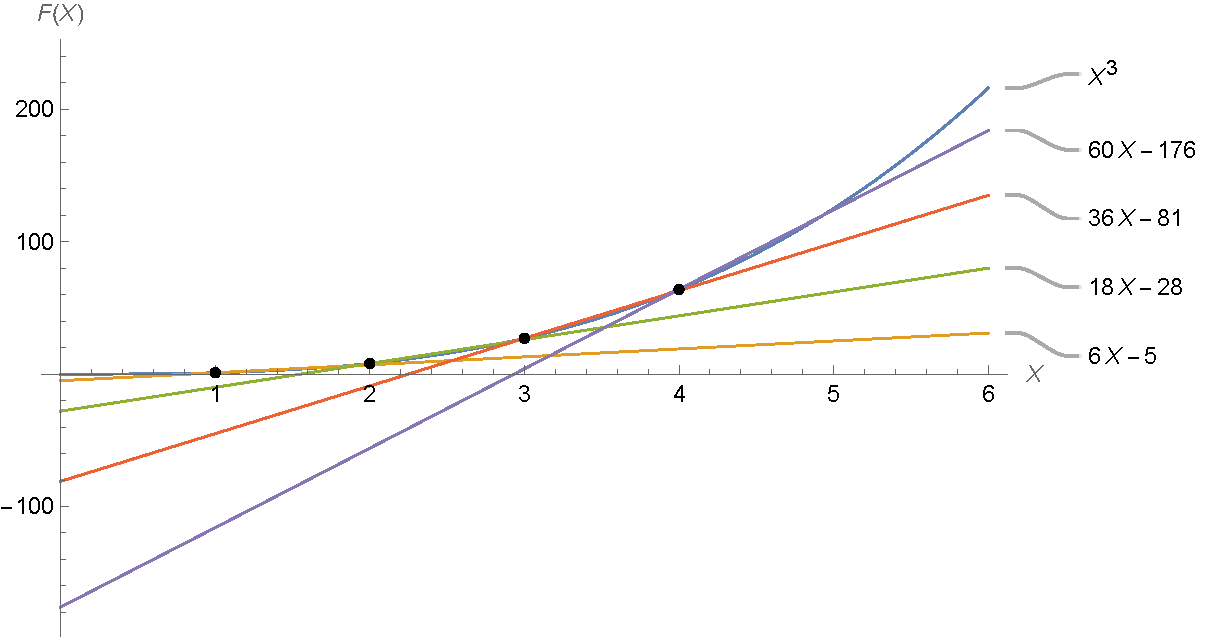
\includegraphics[width=1\textwidth]{sections/images/01_cubes_with_p_1_n_k}
    ~\caption{Polynomials P(1, n, k)}\label{fig:figure}
\end{figure}


    \subsection{Polynomials P(1,X,N) plots for N=1 to 4}
    \begin{figure}[H]
    \centering
    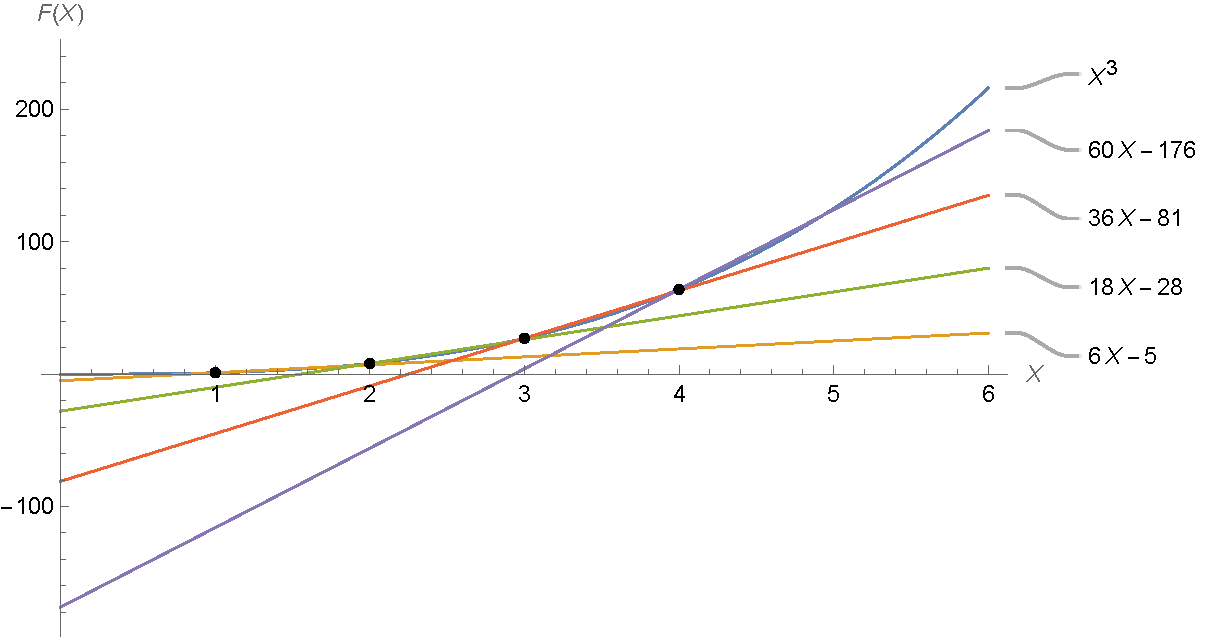
\includegraphics[width=1\textwidth]{sections/images/01_cubes_with_p_1_n_k}
    ~\caption{Polynomials P(1, n, k)}\label{fig:figure}
\end{figure}


    \subsection{Polynomial P(1,X,N) Table of values for N = 6}
    % Table for X, X^3, 126X-540, Diff, and ABS Error %
\begin{table}[h!]
    \centering
    \caption{Comparison of $X^3$, $\polynomialP{1}{X}{6} = 126X-540$, Difference, and Absolute Error Percentage}
    \begin{tabular}{|c|c|c|c|c|}
        \hline
        \textbf{X} & \textbf{$X^3$} & \textbf{$126X-540$} & \textbf{Diff} & \textbf{ABS Error \%} \\ \hline
        5.3        & 148.877        & 127.800             & 21.077        & 14.1573               \\ \hline
        5.4        & 157.464        & 140.400             & 17.064        & 10.8368               \\ \hline
        5.5        & 166.375        & 153.000             & 13.375        & 8.0391                \\ \hline
        5.6        & 175.616        & 165.600             & 10.016        & 5.7034                \\ \hline
        5.7        & 185.193        & 178.200             & 6.993         & 3.7761                \\ \hline
        5.8        & 195.112        & 190.800             & 4.312         & 2.2100                \\ \hline
        5.9        & 205.379        & 203.400             & 1.979         & 0.9636                \\ \hline
        6.0        & 216.000        & 216.000             & 0.000         & 0.0000                \\ \hline
        6.1        & 226.981        & 228.600             & -1.619        & 0.7133                \\ \hline
        6.2        & 238.328        & 241.200             & -2.872        & 1.2051                \\ \hline
        6.3        & 250.047        & 253.800             & -3.753        & 1.5009                \\ \hline
        6.4        & 262.144        & 266.400             & -4.256        & 1.6235                \\ \hline
        6.5        & 274.625        & 279.000             & -4.375        & 1.5931                \\ \hline
        6.6        & 287.496        & 291.600             & -4.104        & 1.4275                \\ \hline
        6.7        & 300.763        & 304.200             & -3.437        & 1.1428                \\ \hline
        6.8        & 314.432        & 316.800             & -2.368        & 0.7531                \\ \hline
        6.9        & 328.509        & 329.400             & -0.891        & 0.2712                \\ \hline
        7.0        & 343.000        & 342.000             & 1.000         & 0.2915                \\ \hline
        7.1        & 357.911        & 354.600             & 3.311         & 0.9251                \\ \hline
        7.2        & 373.248        & 367.200             & 6.048         & 1.6204                \\ \hline
        7.3        & 389.017        & 379.800             & 9.217         & 2.3693                \\ \hline
        7.4        & 405.224        & 392.400             & 12.824        & 3.1647                \\ \hline
        7.5        & 421.875        & 405.000             & 16.875        & 4.0000                \\ \hline
        7.6        & 438.976        & 417.600             & 21.376        & 4.8695                \\ \hline
        7.7        & 456.533        & 430.200             & 26.333        & 5.7680                \\ \hline
        7.8        & 474.552        & 442.800             & 31.752        & 6.6909                \\ \hline
        7.9        & 493.039        & 455.400             & 37.639        & 7.6341                \\ \hline
        8.0        & 512.000        & 468.000             & 44.000        & 8.5938                \\ \hline
        8.1        & 531.441        & 480.600             & 50.841        & 9.5666                \\ \hline
        8.2        & 551.368        & 493.200             & 58.168        & 10.5498               \\ \hline
    \end{tabular}\label{tab:table}
\end{table}



    \subsection{Polynomials Q(1,n,k)}
    \begin{align*}
    \polynomialQ{1}{X}{0} &= 0 \\
    \polynomialQ{1}{X}{1} &= 1 \\
    \polynomialQ{1}{X}{2} &= 6X - 4 \\
    \polynomialQ{1}{X}{3} &= 18X - 27 \\
    \polynomialQ{1}{X}{4} &= 36X - 80 \\
    \polynomialQ{1}{X}{5} &= 60X - 175 \\
    \polynomialQ{1}{X}{6} &= 90X - 324 \\
    \polynomialQ{1}{X}{7} &= 126X - 539 \\
    \polynomialQ{1}{X}{8} &= 168X - 832 \\
    \polynomialQ{1}{X}{9} &= 216X - 1215 \\
    \polynomialQ{1}{X}{10} &= 270X - 1700 \\
    \polynomialQ{1}{X}{11} &= 330X - 2299 \\
    \polynomialQ{1}{X}{12} &= 396X - 3024 \\
    \polynomialQ{1}{X}{13} &= 468X - 3887 \\
    \polynomialQ{1}{X}{14} &= 546X - 4900 \\
    \polynomialQ{1}{X}{15} &= 630X - 6075 \\
    \polynomialQ{1}{X}{16} &= 720X - 7424 \\
    \polynomialQ{1}{X}{17} &= 816X - 8959 \\
    \polynomialQ{1}{X}{18} &= 918X - 10692 \\
    \polynomialQ{1}{X}{19} &= 1026X - 12635 \\
    \polynomialQ{1}{X}{20} &= 1140X - 14800
\end{align*}
\begin{figure}[H]
    \centering
    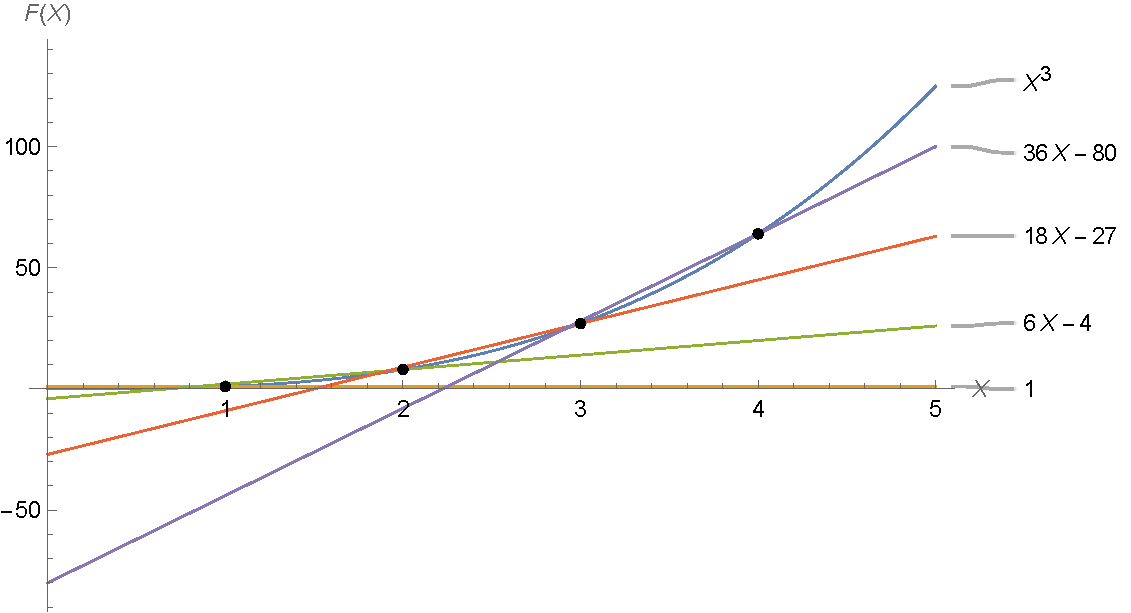
\includegraphics[width=1\textwidth]{sections/images/02_cubes_with_q_1_n_k}
    ~\caption{Polynomials Q(1, n, k)}\label{fig:figure2}
\end{figure}



    \subsection{Polynomial Q(1,n,k) Table n = 6}
    % Table with values of X, X^3, and 90X - 324
\begin{table}[h!]
    \centering
    \caption{Values of $X^3$ and $90X - 324$ for selected $X$}
    \begin{tabular}{|c|c|c|}
        \hline
        \textbf{X} & \textbf{$X^3$} & \textbf{$90X - 324$} \\ \hline
        4.0        & 64.000         & 36.000               \\ \hline
        4.1        & 68.921         & 45.000               \\ \hline
        4.2        & 74.088         & 54.000               \\ \hline
        4.3        & 79.507         & 63.000               \\ \hline
        4.4        & 85.184         & 72.000               \\ \hline
        4.5        & 91.125         & 81.000               \\ \hline
        4.6        & 97.336         & 90.000               \\ \hline
        4.7        & 103.823        & 99.000               \\ \hline
        4.8        & 110.592        & 108.000              \\ \hline
        4.9        & 117.649        & 117.000              \\ \hline
        5.0        & 125.000        & 126.000              \\ \hline
        5.1        & 132.651        & 135.000              \\ \hline
        5.2        & 140.608        & 144.000              \\ \hline
        5.3        & 148.877        & 153.000              \\ \hline
        5.4        & 157.464        & 162.000              \\ \hline
        5.5        & 166.375        & 171.000              \\ \hline
        5.6        & 175.616        & 180.000              \\ \hline
        5.7        & 185.193        & 189.000              \\ \hline
        5.8        & 195.112        & 198.000              \\ \hline
        5.9        & 205.379        & 207.000              \\ \hline
        6.0        & 216.000        & 216.000              \\ \hline
        6.1        & 226.981        & 225.000              \\ \hline
        6.2        & 238.328        & 234.000              \\ \hline
        6.3        & 250.047        & 243.000              \\ \hline
        6.4        & 262.144        & 252.000              \\ \hline
        6.5        & 274.625        & 261.000              \\ \hline
        6.6        & 287.496        & 270.000              \\ \hline
        6.7        & 300.763        & 279.000              \\ \hline
        6.8        & 314.432        & 288.000              \\ \hline
        6.9        & 328.509        & 297.000              \\ \hline
        7.0        & 343.000        & 306.000              \\ \hline
    \end{tabular}\label{tab:table4}
\end{table}


    \subsection{Polynomials P(2,n,k)}
    \begin{align*}
    \polynomialP{2}{X}{0} &= 0 \\
    \polynomialP{2}{X}{1} &= 30X^2 - 60X + 31 \\
    \polynomialP{2}{X}{2} &= 150X^2 - 540X + 512 \\
    \polynomialP{2}{X}{3} &= 420X^2 - 2160X + 2943 \\
    \polynomialP{2}{X}{4} &= 900X^2 - 6000X + 10624 \\
    \polynomialP{2}{X}{5} &= 1650X^2 - 13500X + 29375 \\
    \polynomialP{2}{X}{6} &= 2730X^2 - 26460X + 68256 \\
    \polynomialP{2}{X}{7} &= 4200X^2 - 47040X + 140287 \\
    \polynomialP{2}{X}{8} &= 6120X^2 - 77760X + 263168 \\
    \polynomialP{2}{X}{9} &= 8550X^2 - 121500X + 459999 \\
    \polynomialP{2}{X}{10} &= 11550X^2 - 181500X + 760000 \\
    \polynomialP{2}{X}{11} &= 15180X^2 - 261360X + 1199231 \\
    \polynomialP{2}{X}{12} &= 19500X^2 - 365040X + 1821312 \\
    \polynomialP{2}{X}{13} &= 24570X^2 - 496860X + 2678143 \\
    \polynomialP{2}{X}{14} &= 30450X^2 - 661500X + 3830624 \\
    \polynomialP{2}{X}{15} &= 37200X^2 - 864000X + 5349375 \\
    \polynomialP{2}{X}{16} &= 44880X^2 - 1109760X + 7315456 \\
    \polynomialP{2}{X}{17} &= 53550X^2 - 1404540X + 9821087 \\
    \polynomialP{2}{X}{18} &= 63270X^2 - 1754460X + 12970368 \\
    \polynomialP{2}{X}{19} &= 74100X^2 - 2166000X + 16879999 \\
    \polynomialP{2}{X}{20} &= 86100X^2 - 2646000X + 21680000
\end{align*}
\begin{figure}[H]
    \centering
    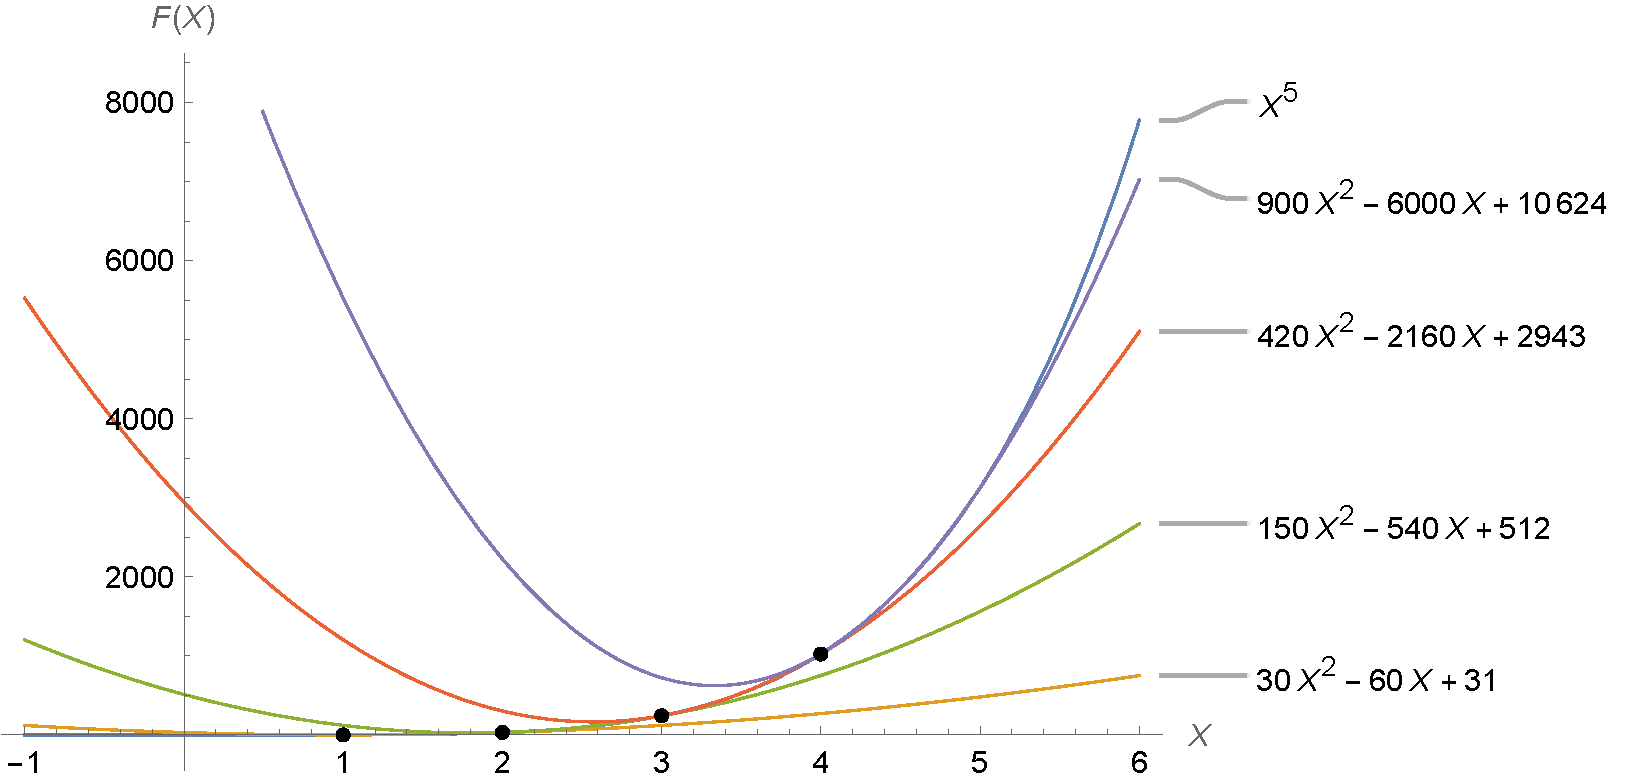
\includegraphics[width=1\textwidth]{sections/images/03_fifth_power_with_p_1_n_k}
    ~\caption{Polynomials P(2, n, k)}\label{fig:figure3}
\end{figure}


    \subsection{Polynomial P(2,n,k) Table n = 4}
    % Table with values of X, X^5, and 900X^2 - 6000X + 10624
\begin{table}[h!]
    \centering
    \caption{Values of $X^5$ and $900X^2 - 6000X + 10624$ for selected $X$}
    \begin{tabular}{|c|c|c|}
        \hline
        \textbf{X} & \textbf{$X^5$} & \textbf{$900X^2 - 6000X + 10624$} \\ \hline
%        3.0        & 243.000        & 724.000                           \\ \hline
%        3.1        & 286.292        & 673.000                           \\ \hline
%        3.2        & 335.544        & 640.000                           \\ \hline
%        3.3        & 391.354        & 625.000                           \\ \hline
%        3.4        & 454.354        & 628.000                           \\ \hline
        3.5        & 525.219        & 649.000                           \\ \hline
        3.6        & 604.662        & 688.000                           \\ \hline
        3.7        & 693.440        & 745.000                           \\ \hline
        3.8        & 792.352        & 820.000                           \\ \hline
        3.9        & 902.242        & 913.000                           \\ \hline
        4.0        & 1024.000       & 1024.000                          \\ \hline
        4.1        & 1158.560       & 1153.000                          \\ \hline
        4.2        & 1306.910       & 1300.000                          \\ \hline
        4.3        & 1470.080       & 1465.000                          \\ \hline
        4.4        & 1649.160       & 1648.000                          \\ \hline
        4.5        & 1845.280       & 1849.000                          \\ \hline
        4.6        & 2059.630       & 2068.000                          \\ \hline
        4.7        & 2293.450       & 2305.000                          \\ \hline
        4.8        & 2548.040       & 2560.000                          \\ \hline
        4.9        & 2824.750       & 2833.000                          \\ \hline
        5.0        & 3125.000       & 3124.000                          \\ \hline
        5.1        & 3450.250       & 3433.000                          \\ \hline
        5.2        & 3802.040       & 3760.000                          \\ \hline
        5.3        & 4181.950       & 4105.000                          \\ \hline
        5.4        & 4591.650       & 4468.000                          \\ \hline
        5.5        & 5032.840       & 4849.000                          \\ \hline
%        5.6        & 5507.320       & 5248.000                          \\ \hline
%        5.7        & 6016.920       & 5665.000                          \\ \hline
%        5.8        & 6563.570       & 6100.000                          \\ \hline
%        5.9        & 7149.240       & 6553.000                          \\ \hline
%        6.0        & 7776.000       & 7024.000                          \\ \hline
    \end{tabular}\label{tab:table2}
\end{table}


    \subsection{Polynomials Q(2,n,k)}
    \begin{align*}
    \polynomialQ{2}{N}{0} &= 0 \\
    \polynomialQ{2}{N}{1} &= 1 \\
    \polynomialQ{2}{N}{2} &= 30N^2 - 60N + 32 \\
    \polynomialQ{2}{N}{3} &= 150N^2 - 540N + 513 \\
    \polynomialQ{2}{N}{4} &= 420N^2 - 2160N + 2944 \\
    \polynomialQ{2}{N}{5} &= 900N^2 - 6000N + 10625 \\
    \polynomialQ{2}{N}{6} &= 1650N^2 - 13500N + 29376 \\
    \polynomialQ{2}{N}{7} &= 2730N^2 - 26460N + 68257 \\
    \polynomialQ{2}{N}{8} &= 4200N^2 - 47040N + 140288 \\
    \polynomialQ{2}{N}{9} &= 6120N^2 - 77760N + 263169 \\
    \polynomialQ{2}{N}{10} &= 8550N^2 - 121500N + 460000 \\
    \polynomialQ{2}{N}{11} &= 11550N^2 - 181500N + 760001 \\
    \polynomialQ{2}{N}{12} &= 15180N^2 - 261360N + 1199232 \\
    \polynomialQ{2}{N}{13} &= 19500N^2 - 365040N + 1821313 \\
    \polynomialQ{2}{N}{14} &= 24570N^2 - 496860N + 2678144 \\
    \polynomialQ{2}{N}{15} &= 30450N^2 - 661500N + 3830625 \\
    \polynomialQ{2}{N}{16} &= 37200N^2 - 864000N + 5349376 \\
    \polynomialQ{2}{N}{17} &= 44880N^2 - 1109760N + 7315457 \\
    \polynomialQ{2}{N}{18} &= 53550N^2 - 1404540N + 9821088 \\
    \polynomialQ{2}{N}{19} &= 63270N^2 - 1754460N + 12970369 \\
    \polynomialQ{2}{N}{20} &= 74100N^2 - 2166000N + 16880000
\end{align*}
\begin{figure}[H]
    \centering
    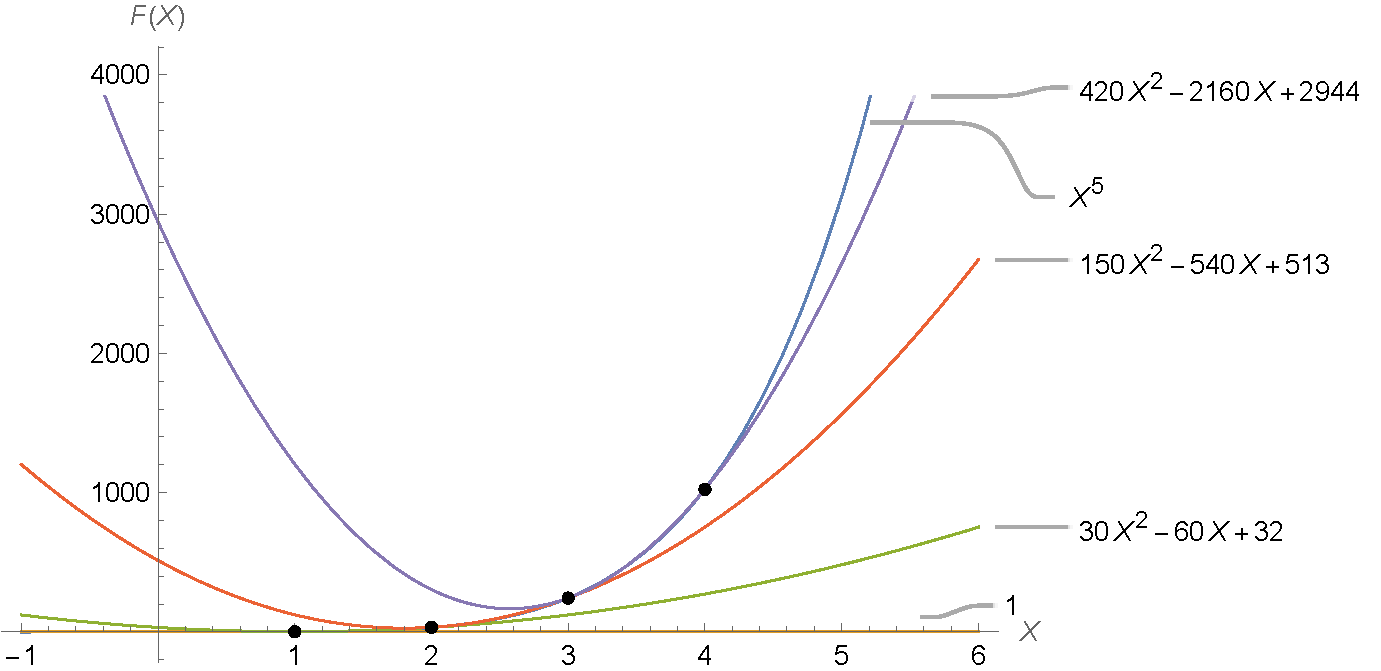
\includegraphics[width=1\textwidth]{sections/images/04_fifth_power_with_q_1_n_k}
    ~\caption{Polynomials P(2, n, k)}\label{fig:figure4}
\end{figure}


    \subsection{Polynomial Q(2,n,k) Table n = 4}
    % Table with values of X, X^5, and 420X^2 - 2160X + 2944
\begin{table}[h!]
    \centering
    \caption{Values of $X^5$ and $420X^2 - 2160X + 2944$ for selected $X$}
    \begin{tabular}{|c|c|c|}
        \hline
        \textbf{X} & \textbf{$X^5$} & \textbf{$420X^2 - 2160X + 2944$} \\ \hline
        2.0        & 32.000         & 304.000                          \\ \hline
        2.1        & 40.841         & 260.200                          \\ \hline
        2.2        & 51.536         & 224.800                          \\ \hline
        2.3        & 64.363         & 197.800                          \\ \hline
        2.4        & 79.626         & 179.200                          \\ \hline
        2.5        & 97.656         & 169.000                          \\ \hline
        2.6        & 118.814        & 167.200                          \\ \hline
        2.7        & 143.489        & 173.800                          \\ \hline
        2.8        & 172.104        & 188.800                          \\ \hline
        2.9        & 205.111        & 212.200                          \\ \hline
        3.0        & 243.000        & 244.000                          \\ \hline
        3.1        & 286.292        & 284.200                          \\ \hline
        3.2        & 335.544        & 332.800                          \\ \hline
        3.3        & 391.354        & 389.800                          \\ \hline
        3.4        & 454.354        & 455.200                          \\ \hline
        3.5        & 525.219        & 529.000                          \\ \hline
        3.6        & 604.662        & 611.200                          \\ \hline
        3.7        & 693.440        & 701.800                          \\ \hline
        3.8        & 792.352        & 800.800                          \\ \hline
        3.9        & 902.242        & 908.200                          \\ \hline
        4.0        & 1024.000       & 1024.000                         \\ \hline
        4.1        & 1158.560       & 1148.200                         \\ \hline
        4.2        & 1306.910       & 1280.800                         \\ \hline
        4.3        & 1470.080       & 1421.800                         \\ \hline
        4.4        & 1649.160       & 1571.200                         \\ \hline
        4.5        & 1845.280       & 1729.000                         \\ \hline
        4.6        & 2059.630       & 1895.200                         \\ \hline
        4.7        & 2293.450       & 2069.800                         \\ \hline
        4.8        & 2548.040       & 2252.800                         \\ \hline
        4.9        & 2824.750       & 2444.200                         \\ \hline
        5.0        & 3125.000       & 2644.000                         \\ \hline
    \end{tabular}\label{tab:table5}
\end{table}


    \subsection{Polynomials P(3,n,k)}
    \begin{align*}
    \polynomialP{3}{X}{0} &= 0 \\
    \polynomialP{3}{X}{1} &= 140X^3 - 420X^2 + 406X - 125 \\
    \polynomialP{3}{X}{2} &= 1260X^3 - 7140X^2 + 13818X - 9028 \\
    \polynomialP{3}{X}{3} &= 5040X^3 - 41160X^2 + 115836X - 110961 \\
    \polynomialP{3}{X}{4} &= 14000X^3 - 148680X^2 + 545860X - 684176 \\
    \polynomialP{3}{X}{5} &= 31500X^3 - 411180X^2 + 1858290X - 2871325 \\
    \polynomialP{3}{X}{6} &= 61740X^3 - 955500X^2 + 5124126X - 9402660 \\
    \polynomialP{3}{X}{7} &= 109760X^3 - 1963920X^2 + 12182968X - 25872833 \\
    \polynomialP{3}{X}{8} &= 181440X^3 - 3684240X^2 + 25945416X - 62572096 \\
    \polynomialP{3}{X}{9} &= 283500X^3 - 6439860X^2 + 50745870X - 136972701 \\
    \polynomialP{3}{X}{10} &= 423500X^3 - 10639860X^2 + 92745730X - 276971300 \\
    \polynomialP{3}{X}{11} &= 609840X^3 - 16789080X^2 + 160386996X - 524988145 \\
    \polynomialP{3}{X}{12} &= 851760X^3 - 25498200X^2 + 264896268X - 943023888 \\
    \polynomialP{3}{X}{13} &= 1159340X^3 - 37493820X^2 + 420839146X - 1618774781 \\
    \polynomialP{3}{X}{14} &= 1543500X^3 - 53628540X^2 + 646725030X - 2672907076 \\
    \polynomialP{3}{X}{15} &= 2016000X^3 - 74891040X^2 + 965662320X - 4267591425 \\
    \polynomialP{3}{X}{16} &= 2589440X^3 - 102416160X^2 + 1406064016X - 6616398080 \\
    \polynomialP{3}{X}{17} &= 3277260X^3 - 137494980X^2 + 2002403718X - 9995653693 \\
    \polynomialP{3}{X}{18} &= 4093740X^3 - 181584900X^2 + 2796022026X - 14757360516 \\
    \polynomialP{3}{X}{19} &= 5054000X^3 - 236319720X^2 + 3835983340X - 21343778801 \\
    \polynomialP{3}{X}{20} &= 6174000X^3 - 303519720X^2 + 5179983060X - 30303773200
\end{align*}
\begin{figure}[H]
    \centering
    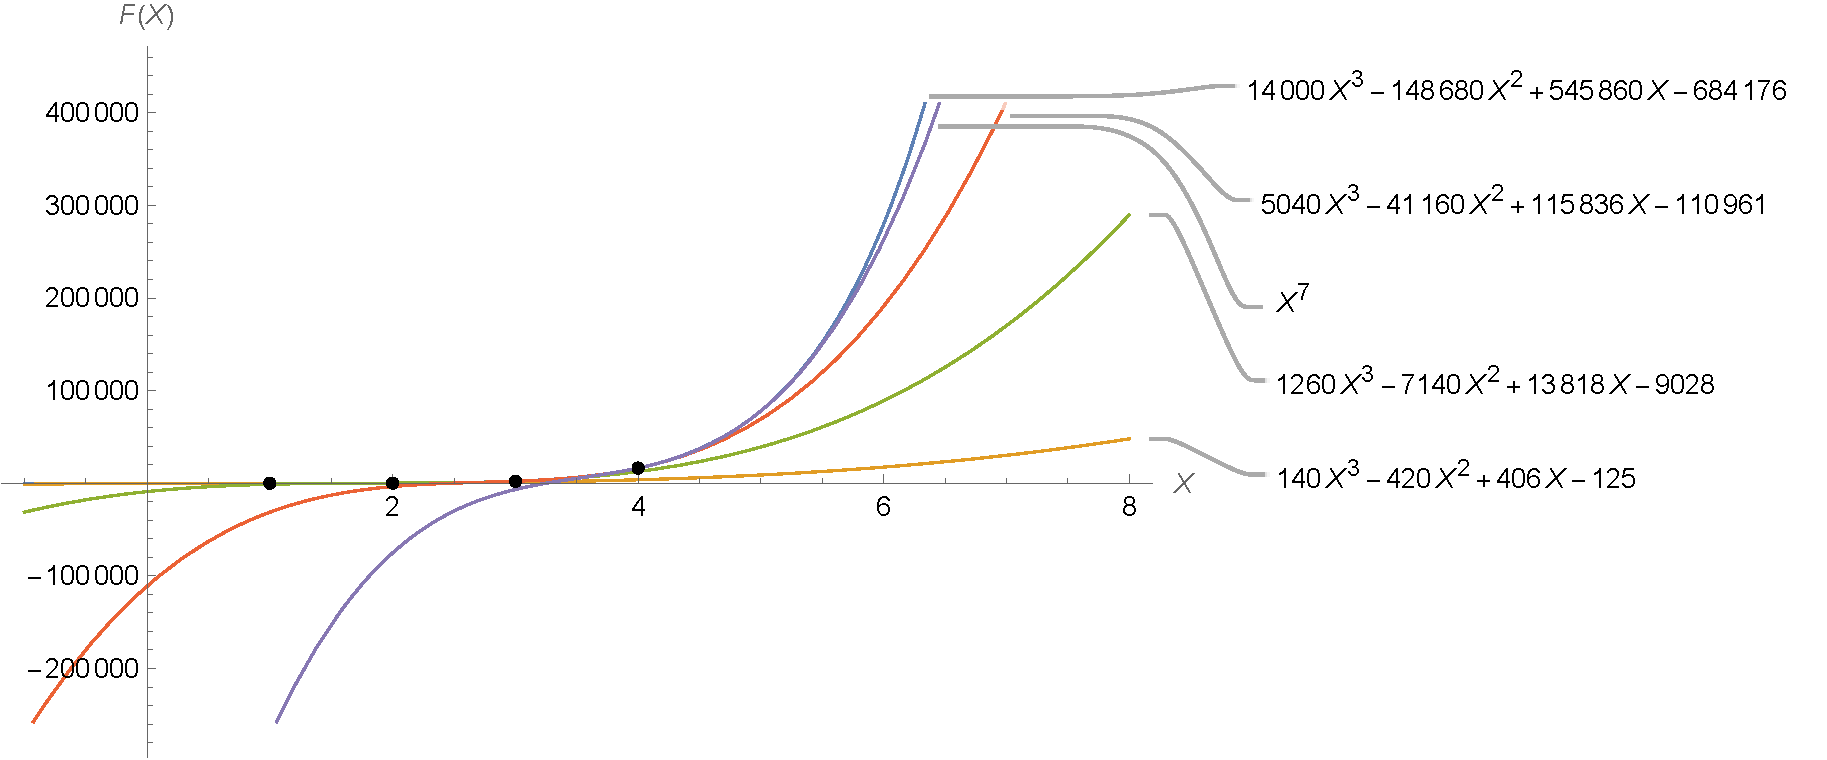
\includegraphics[width=1\textwidth]{sections/images/05_seventh_power_with_p_3_n_k}
    ~\caption{Polynomials P(1, n, k)}\label{fig:figure5}
\end{figure}


    \subsection{Polynomial P(3,n,k) Table n = 3}
    % Table with values of X, X^7, and 5040X^3 - 41160X^2 + 115836X - 110961
\begin{table}[h!]
    \centering
    \caption{Values of $X^7$ and $5040X^3 - 41160X^2 + 115836X - 110961$ for selected $X$}
    \begin{tabular}{|c|c|c|}
        \hline
        \textbf{X} & \textbf{$X^7$} & \textbf{$5040X^3 - 41160X^2 + 115836X - 110961$} \\ \hline
        2.0        & 128.000        & -3609.000                                        \\ \hline
        2.1        & 180.109        & -2545.560                                        \\ \hline
        2.2        & 249.436        & -1670.280                                        \\ \hline
        2.3        & 340.483        & -952.920                                         \\ \hline
        2.4        & 458.647        & -363.240                                         \\ \hline
        2.5        & 610.352        & 129.000                                          \\ \hline
        2.6        & 803.181        & 554.040                                          \\ \hline
        2.7        & 1046.040       & 942.120                                          \\ \hline
        2.8        & 1349.290       & 1323.480                                         \\ \hline
        2.9        & 1724.990       & 1728.360                                         \\ \hline
        3.0        & 2187.000       & 2187.000                                         \\ \hline
        3.1        & 2751.260       & 2729.640                                         \\ \hline
        3.2        & 3435.970       & 3386.520                                         \\ \hline
        3.3        & 4261.840       & 4187.880                                         \\ \hline
        3.4        & 5252.340       & 5163.960                                         \\ \hline
        3.5        & 6433.930       & 6345.000                                         \\ \hline
        3.6        & 7836.420       & 7761.240                                         \\ \hline
        3.7        & 9493.190       & 9442.920                                         \\ \hline
        3.8        & 11441.600      & 11420.300                                        \\ \hline
        3.9        & 13723.100      & 13723.600                                        \\ \hline
        4.0        & 16384.000      & 16383.000                                        \\ \hline
        4.1        & 19475.400      & 19428.800                                        \\ \hline
        4.2        & 23053.900      & 22891.300                                        \\ \hline
        4.3        & 27181.900      & 26800.700                                        \\ \hline
        4.4        & 31927.800      & 31187.200                                        \\ \hline
        4.5        & 37366.900      & 36081.000                                        \\ \hline
        4.6        & 43581.800      & 41512.400                                        \\ \hline
        4.7        & 50662.300      & 47511.700                                        \\ \hline
        4.8        & 58706.800      & 54109.100                                        \\ \hline
        4.9        & 67822.300      & 61334.800                                        \\ \hline
        5.0        & 78125.000      & 69219.000                                        \\ \hline
    \end{tabular}\label{tab:table3}
\end{table}


    \subsection{Polynomials Q(3,n,k)}
    \begin{align*}
    \polynomialQ{3}{N}{0} &= 0 \\
    \polynomialQ{3}{N}{1} &= 1 \\
    \polynomialQ{3}{N}{2} &= 140N^3 - 420N^2 + 406N - 124 \\
    \polynomialQ{3}{N}{3} &= 1260N^3 - 7140N^2 + 13818N - 9027 \\
    \polynomialQ{3}{N}{4} &= 5040N^3 - 41160N^2 + 115836N - 110960 \\
    \polynomialQ{3}{N}{5} &= 14000N^3 - 148680N^2 + 545860N - 684175 \\
    \polynomialQ{3}{N}{6} &= 31500N^3 - 411180N^2 + 1858290N - 2871324 \\
    \polynomialQ{3}{N}{7} &= 61740N^3 - 955500N^2 + 5124126N - 9402659 \\
    \polynomialQ{3}{N}{8} &= 109760N^3 - 1963920N^2 + 12182968N - 25872832 \\
    \polynomialQ{3}{N}{9} &= 181440N^3 - 3684240N^2 + 25945416N - 62572095 \\
    \polynomialQ{3}{N}{10} &= 283500N^3 - 6439860N^2 + 50745870N - 136972700 \\
    \polynomialQ{3}{N}{11} &= 423500N^3 - 10639860N^2 + 92745730N - 276971299 \\
    \polynomialQ{3}{N}{12} &= 609840N^3 - 16789080N^2 + 160386996N - 524988144 \\
    \polynomialQ{3}{N}{13} &= 851760N^3 - 25498200N^2 + 264896268N - 943023887 \\
    \polynomialQ{3}{N}{14} &= 1159340N^3 - 37493820N^2 + 420839146N - 1618774780 \\
    \polynomialQ{3}{N}{15} &= 1543500N^3 - 53628540N^2 + 646725030N - 2672907075 \\
    \polynomialQ{3}{N}{16} &= 2016000N^3 - 74891040N^2 + 965662320N - 4267591424 \\
    \polynomialQ{3}{N}{17} &= 2589440N^3 - 102416160N^2 + 1406064016N - 6616398079 \\
    \polynomialQ{3}{N}{18} &= 3277260N^3 - 137494980N^2 + 2002403718N - 9995653692 \\
    \polynomialQ{3}{N}{19} &= 4093740N^3 - 181584900N^2 + 2796022026N - 14757360515 \\
    \polynomialQ{3}{N}{20} &= 5054000N^3 - 236319720N^2 + 3835983340N - 21343778800 \\
\end{align*}
\begin{figure}[H]
    \centering
    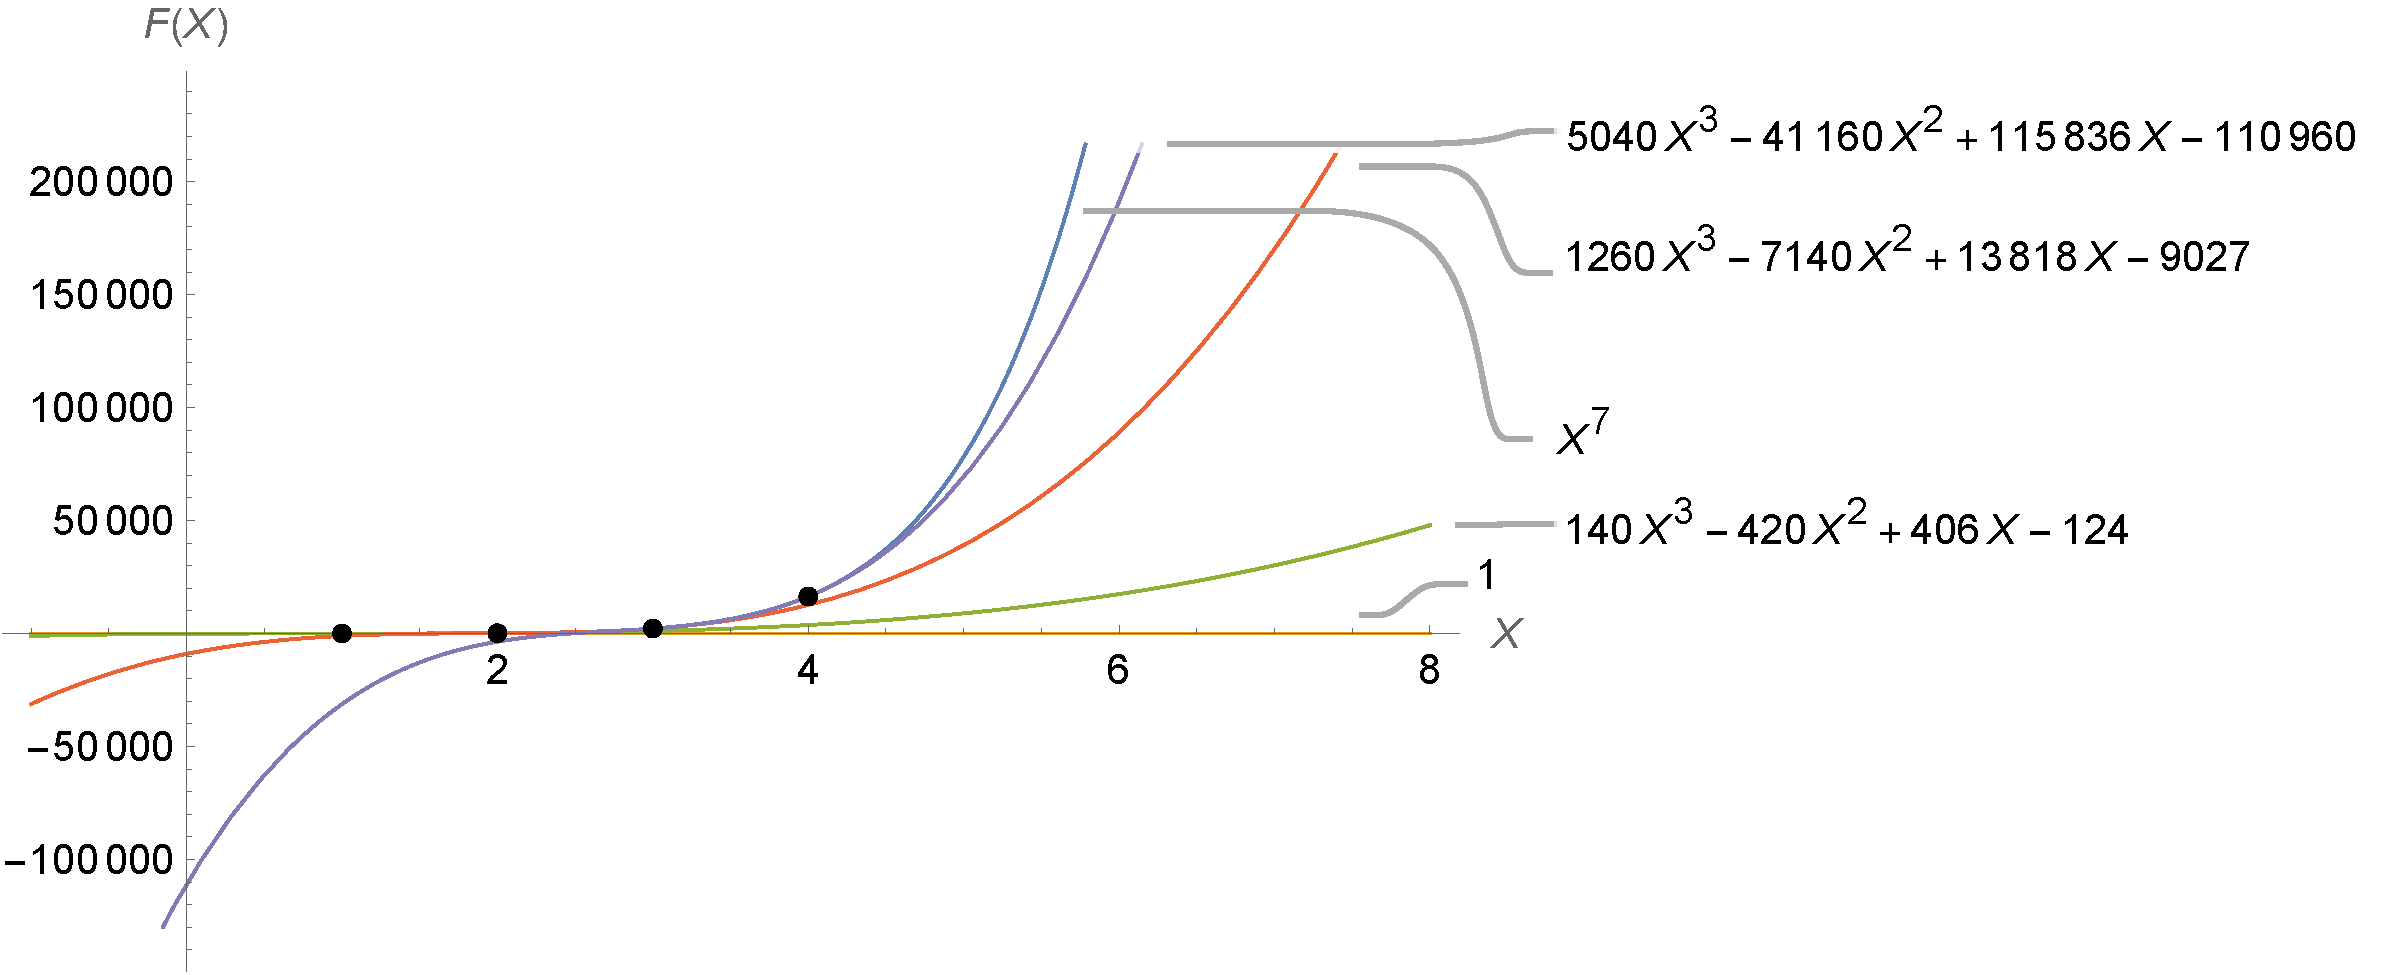
\includegraphics[width=1\textwidth]{sections/images/06_seventh_power_with_q_3_n_k}
    ~\caption{Polynomials P(1, n, k)}\label{fig:figure6}
\end{figure}


    \subsection{Polynomial Q(3,n,k) Table n = 3}
    \begin{table}[h!]
    \centering
    \caption{Comparison of $X^7$, $\polynomialP{3}{X}{3} = 1260X^3 - 7140X^2 + 13818X - 9027$, Difference, and Absolute Error Percentage}
    \begin{tabular}{|c|c|c|c|c|}
        \hline
        \textbf{X} & $X^7$   & $1260X^3 - 7140X^2 + 13818X - 9027$ & \textbf{Diff} & \textbf{ABS Error \%} \\ \hline
        1.6        & 26.8435 & -35.64                              & 62.4835       & 232.769               \\ \hline
        1.7        & 41.0339 & 19.38                               & 21.6539       & 52.7707               \\ \hline
        1.8        & 61.222  & 60.12                               & 1.102         & 1.80001               \\ \hline
        1.9        & 89.3872 & 94.14                               & -4.75283      & 5.31712               \\ \hline
        2.0        & 128.0   & 129.0                               & -1.0          & 0.78125               \\ \hline
        2.1        & 180.109 & 172.26                              & 7.84885       & 4.35784               \\ \hline
        2.2        & 249.436 & 231.48                              & 17.9558       & 7.19856               \\ \hline
        2.3        & 340.483 & 314.22                              & 26.2625       & 7.71333               \\ \hline
        2.4        & 458.647 & 428.04                              & 30.6071       & 6.67335               \\ \hline
        2.5        & 610.352 & 580.5                               & 29.8516       & 4.89088               \\ \hline
        2.6        & 803.181 & 779.16                              & 24.021        & 2.99074               \\ \hline
        2.7        & 1046.04 & 1031.58                             & 14.4553       & 1.38192               \\ \hline
        2.8        & 1349.29 & 1345.32                             & 3.97285       & 0.29444               \\ \hline
        2.9        & 1724.99 & 1727.94                             & -2.95237      & 0.171153              \\ \hline
        3.0        & 2187.0  & 2187.0                              & 0.0           & 0.0                   \\ \hline
        3.1        & 2751.26 & 2730.06                             & 21.2014       & 0.770607              \\ \hline
        3.2        & 3435.97 & 3364.68                             & 71.2938       & 2.07492               \\ \hline
        3.3        & 4261.84 & 4098.42                             & 163.424       & 3.83459               \\ \hline
        3.4        & 5252.34 & 4938.84                             & 313.495       & 5.96868               \\ \hline
        3.5        & 6433.93 & 5893.5                              & 540.43        & 8.39968               \\ \hline
        3.6        & 7836.42 & 6969.96                             & 866.456       & 11.0568               \\ \hline
        3.7        & 9493.19 & 8175.78                             & 1317.41       & 13.8774               \\ \hline
    \end{tabular}\label{tab:table6}
\end{table}



%    \bibliographystyle{unsrt}
%    \bibliography{PlotsOfClosedForms}

\end{document}
